\documentclass[border=4pt]{standalone}
\usepackage{lmodern}
\usepackage{amsmath,amssymb}
\usepackage{pgfplots}
\pgfplotsset{compat=1.18}
\begin{document}
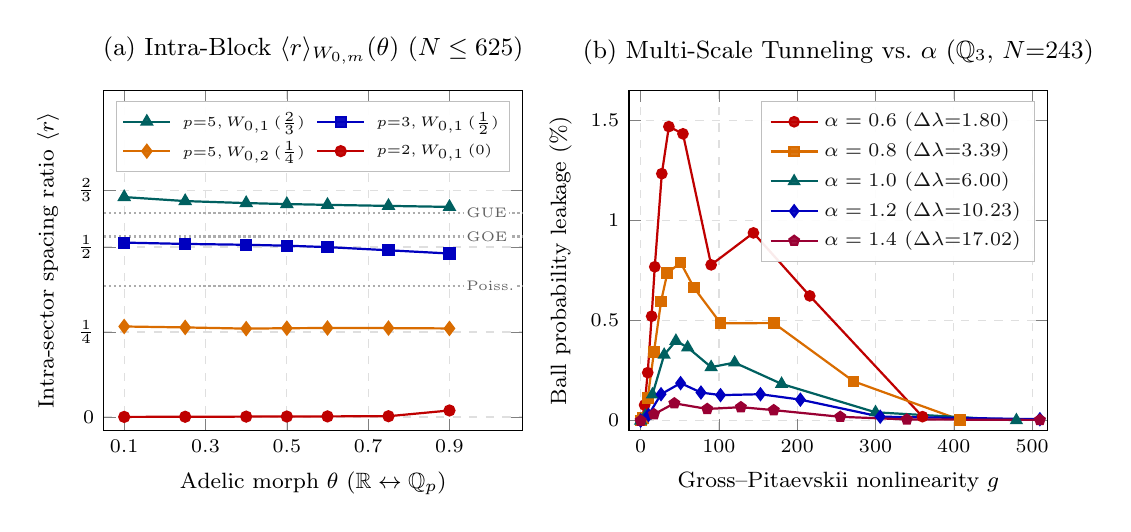
\begin{tikzpicture}
\begin{axis}[
  name=leftplot,
  width=6.9cm,
  height=5.9cm,
  title={\small (a) Intra-Block $\langle r \rangle_{W_{0,m}}(\theta)$ ($N \le 625$)},
  xlabel={Adelic morph $\theta$ ($\mathbb{R} \leftrightarrow \mathbb{Q}_p$)},
  ylabel={Intra-sector spacing ratio $\langle r \rangle$},
  xmin=0.05, xmax=1.08,
  ymin=-0.04, ymax=0.96,
  xtick={0.1,0.3,0.5,0.7,0.9},
  ytick={0,0.25,0.5,0.6667},
  yticklabels={$0$,$\tfrac{1}{4}$,$\tfrac{1}{2}$,$\tfrac{2}{3}$},
  grid=major,
  grid style={dashed, gray!25},
  legend style={at={(0.50,0.97)}, anchor=north, legend columns=2, column sep=2pt, inner sep=2pt, font=\tiny, fill=white, fill opacity=0.95, draw=gray!50},
  legend cell align=left,
  label style={font=\footnotesize},
  tick label style={font=\scriptsize},
]
  % Random-matrix reference lines
  \addplot[gray!65, densely dotted, thick, forget plot] coordinates {(0.05, 0.5996) (1.08, 0.5996)};
  \node[anchor=west, font=\tiny, text=gray!75!black, fill=white, inner sep=0.8pt] at (axis cs:0.935, 0.600) {GUE};
  \addplot[gray!65, densely dotted, thick, forget plot] coordinates {(0.05, 0.5307) (1.08, 0.5307)};
  \node[anchor=west, font=\tiny, text=gray!75!black, fill=white, inner sep=0.8pt] at (axis cs:0.935, 0.531) {GOE};
  \addplot[gray!65, densely dotted, thick, forget plot] coordinates {(0.05, 0.3863) (1.08, 0.3863)};
  \node[anchor=west, font=\tiny, text=gray!75!black, fill=white, inner sep=0.8pt] at (axis cs:0.935, 0.386) {Poiss.};

  \addplot[color=teal!75!black, thick, mark=triangle*, mark size=2.1pt] coordinates { (0.10, 0.64688) (0.25, 0.63511) (0.40, 0.62919) (0.50, 0.62633) (0.60, 0.62399) (0.75, 0.62092) (0.90, 0.61799) };
  \addlegendentry{$p{=}5,W_{0,1}\,(\tfrac{2}{3})$}
  \addplot[color=blue!75!black, thick, mark=square*, mark size=1.8pt] coordinates { (0.10, 0.51297) (0.25, 0.50906) (0.40, 0.50656) (0.50, 0.50388) (0.60, 0.49976) (0.75, 0.49043) (0.90, 0.48088) };
  \addlegendentry{$p{=}3,W_{0,1}\,(\tfrac{1}{2})$}
  \addplot[color=orange!85!black, thick, mark=diamond*, mark size=2.2pt] coordinates { (0.10, 0.26629) (0.25, 0.26352) (0.40, 0.25999) (0.50, 0.26122) (0.60, 0.26181) (0.75, 0.26152) (0.90, 0.26053) };
  \addlegendentry{$p{=}5,W_{0,2}\,(\tfrac{1}{4})$}
  \addplot[color=red!75!black, thick, mark=*, mark size=1.8pt] coordinates { (0.10, 0.00034) (0.25, 0.00079) (0.40, 0.00121) (0.50, 0.00149) (0.60, 0.00185) (0.75, 0.00239) (0.90, 0.01927) };
  \addlegendentry{$p{=}2,W_{0,1}\,(0)$}
\end{axis}

\begin{axis}[
  at={(leftplot.east)},
  anchor=west,
  xshift=1.35cm,
  width=6.9cm,
  height=5.9cm,
  title={\small (b) Multi-Scale Tunneling vs.\ $\alpha$ ($\mathbb{Q}_3$, $N{=}243$)},
  xlabel={Gross--Pitaevskii nonlinearity $g$},
  ylabel={Ball probability leakage (\%)},
  xmin=-15, xmax=520,
  ymin=-0.05, ymax=1.65,
  grid=major,
  grid style={dashed, gray!25},
  legend pos=north east,
  legend cell align=left,
  legend style={font=\scriptsize, fill=white, fill opacity=0.92, draw=gray!50},
  label style={font=\footnotesize},
  tick label style={font=\scriptsize},
]
  \addplot[color=red!75!black, thick, mark=*, mark size=1.7pt] coordinates { (0, 0.0000) (2, 0.0128) (5, 0.0782) (9, 0.2399) (14, 0.5219) (18, 0.7691) (27, 1.2347) (36, 1.4700) (54, 1.4340) (90, 0.7788) (144, 0.9386) (216, 0.6237) (360, 0.0199) };
  \addlegendentry{$\alpha = 0.6$ ($\Delta\lambda{=}1.80$)}
  \addplot[color=orange!85!black, thick, mark=square*, mark size=1.7pt] coordinates { (0, 0.0000) (3, 0.0136) (9, 0.1145) (17, 0.3434) (26, 0.5955) (34, 0.7375) (51, 0.7898) (68, 0.6650) (102, 0.4870) (170, 0.4876) (272, 0.1965) (408, 0.0040) };
  \addlegendentry{$\alpha = 0.8$ ($\Delta\lambda{=}3.39$)}
  \addplot[color=teal!75!black, thick, mark=triangle*, mark size=2.0pt] coordinates { (0, 0.0000) (6, 0.0240) (15, 0.1305) (30, 0.3288) (45, 0.3987) (60, 0.3661) (90, 0.2674) (120, 0.2901) (180, 0.1836) (300, 0.0416) (480, 0.0015) };
  \addlegendentry{$\alpha = 1.0$ ($\Delta\lambda{=}6.00$)}
  \addplot[color=blue!75!black, thick, mark=diamond*, mark size=2.0pt] coordinates { (0, 0.0000) (10, 0.0282) (26, 0.1322) (51, 0.1875) (77, 0.1405) (102, 0.1275) (153, 0.1321) (204, 0.1050) (306, 0.0198) (510, 0.0072) };
  \addlegendentry{$\alpha = 1.2$ ($\Delta\lambda{=}10.23$)}
  \addplot[color=purple!80!black, thick, mark=pentagon*, mark size=1.8pt] coordinates { (0, 0.0000) (17, 0.0319) (43, 0.0866) (85, 0.0584) (128, 0.0673) (170, 0.0525) (255, 0.0192) (340, 0.0060) (510, 0.0036) };
  \addlegendentry{$\alpha = 1.4$ ($\Delta\lambda{=}17.02$)}
\end{axis}
\end{tikzpicture}
\end{document}
